\section{Symmetrisk og asymmetrisk nøglekryptering og digitale signaturer}

\subsection{Læringsmål}

\begin{itemize}
	\item Redegør for og vis eksempler på symmetrisk og asymmetrisk nøglekryptering, samt
	anvendelsen af disse i digitale signaturer.
	\item Samt forklar hvordan digitale signaturer anvendes og stoles på i praksis.
\end{itemize}

\subsection{Redegør for og vis eksempler på symmetrisk og asymmetrisk nøglekryptering, samt anvendelsen af disse i digitale signaturer}
Ved symmetrisk kryptering skal en nøgle deles på forhånd. Figur~\ref{fig:symmetrickeyenc} illustrerer. En fordel er at metoden er 1.000 til 10.000 gange hurtigere end asymmetrisk. 

\begin{figure}[H]
	\centering
	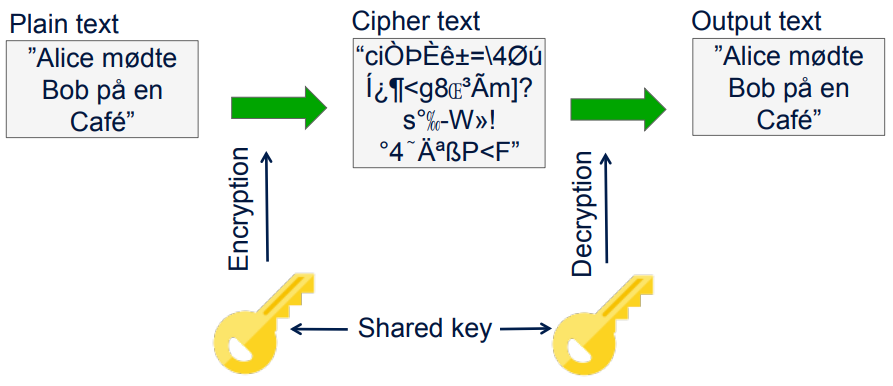
\includegraphics[width=0.8\linewidth]{figs/spm5/symmetric_key_enc}
	\caption{Symmetrisk nøglekryptering}
	\label{fig:symmetrickeyenc}
\end{figure}

Asymmetrisk kryptering af beskrevet i Afsnit~\ref{sec:asymmetric} på Side~\pageref{sec:asymmetric}.

\subsubsection{Matematikken}
Her er \textit{C} ciphertext, \textit{P} plaintext.

\begin{align}
	C &= E(k,P)\\
	P &= D(k,C)
\end{align}

\subsubsection{Cryptographiv Primitives}
Disse grundlæggende blokke bruges til at lave krypteringsalgoritmer.

\paragraph{Substitution}
Udskifter tegn med andre. F.eks. $ABC \Rightarrow 123$

\paragraph{Transposition}
Flytter tegn i strengen. F.eks. $ABC \Rightarrow BCA$

\paragraph{Confusion}
Ændringen af ét tegn ændre hele den resulterende streng.

\paragraph{Diffusion}
Distribuere informationen fra ét tegn ud i hele cifferteksten.

\subsubsection{Anvendelse af kryptering i signature}
Figur~\ref{fig:digital-signature} viser hvordan en digital signatur\footnote{Se \url{https://youtu.be/GSIDS_lvRv4?t=4m2s}} laves.

\begin{figure}[H]
	\centering
	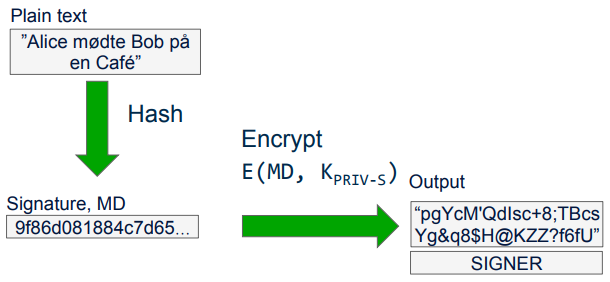
\includegraphics[width=0.7\linewidth]{figs/spm5/digital-signature}
	\caption{Hvordan en besked signeres}
	\label{fig:digital-signature}
\end{figure}

\subsection{Samt forklar hvordan digitale signaturer anvendes og stoles på i praksis}
En digital signatur består af:

\begin{itemize}
	\item En fil
	\item Hvem signatures tilhører
	\item Validering af at signaturen er ægte og ikke forfalsket
	\item Demonstration af at filen ikke er ændret
	\item En forbindelsen mellem signatur og filen
\end{itemize}

\subsection{Public key infrastructure}
Er en række roller, politikker og procedure, som bruges til at oprette, vedligeholde og distribuere m.m. digitale certifikater.

\subsubsection{Elementer i PKI}
For at hele systemet skal virke er infrastruktur med disse elementer bygget: 

\paragraph{Certification Authority (CA)} udsteder, gemmer og signere certifikater.

\paragraph{Registration Authority (RA)} ''voucher'' for identiteten af brugerne overfor en CA.

\paragraph{Repository} er en database med aktive digitale certifikater i et CA system.

\paragraph{Archive} indeholder gamle certifikater, som kan bruges i fremtidige konflikter.

\paragraph{Certificate Revocation Lists (CRLs)} holder på certifikater som er blevet ''revoked''.

\paragraph{Public key certificate} bekræfter at identiteten har de korrekte credentials.

\paragraph{PKI users} organisationer eller individer, som bruger PKI, men som ikke udsteder certifikater.

\subsubsection{Certificate lifecycle}

\begin{enumerate}
	\item \textbf{Issuance}
	\item \textbf{Monitor} - Expiry, Revocation status, Private key
	\item \textbf{Renewal} - Same private key
	\item \textbf{Revocation} - Private key compromised, certificate no longer in use
	\item \textbf{Reissue} - Same expiry data, add/remove name in certicate
	\item \textbf{Rekey} - New private key. Certficate revoked.
\end{enumerate}

\subsubsection{Authentication Methods}

\begin{itemize}
	\item \textbf{Domain Validated (DV)}
	\begin{itemize}
		\item Mail sendt til difineret alias, som admin@
		\item Der oprettes en DNS TXT Record
		\item Der skal ligge en fil på serveren
	\end{itemize}
	\item \textbf{Organisation Validated (OV)}
	\begin{itemize}
		\item Der skal fremsendes dokumenter fra organisationen
		\item Man ringes op
	\end{itemize}
	\item \textbf{Extended Validated (EV)}
	\begin{itemize}
		\item Organisationsdokumenter sendes
		\item Telefonopkald
		\item ''Legal, physical and operatioal existence of the entity''
	\end{itemize}
\end{itemize}
